%  LaTeX support: latex@mdpi.com 
%  For support, please attach all files needed for compiling as well as the log file, and specify your operating system, LaTeX version, and LaTeX editor.

\newcommand{\qsdpapertitle}{Causal Motion Under Planck-Paced Reconfiguration: Inertial Emergence in General Substrate Theory}
\newcommand{\qsdauthorname}{Michael Bush}
\newcommand{\qsdauthorinitials}{M.B.}
\newcommand{\qsdauthoremail}{mbush@haddentechnologies.com}
\newcommand{\qsdorcid}{0009-0003-9747-9109}
\newcommand{\qsdcorp}{Hadden Technologies Corporation}
\newcommand{\qsdgptname}{ChatGPT}
\newcommand{\qsdgptver}{GPT-4o}
\newcommand{\qsdgptyear}{2025}
\newcommand{\qsdkeywords}{General Substrate Theroy,GST,Quantum Substrate Dynamics,QSD,Inertia,Scalar coherence,Substrate dynamics,planck energy,
Phase re-locking,Momentum,Rotational loss,Scalar recovery,Mass-phase,Conserved substrate}
\newcommand{\qsdmethodstatement}
{This work was developed through first-principles modeling using a conserved coherence substrate framework. All derivations were performed structurally, with motion, inertia, and rotational behavior treated as manifestations of scalar phase reconfiguration. Mathematical relationships were constructed to maintain causal consistency and empirical compatibility, while avoiding reliance on classical axioms such as intrinsic mass or force. The method emphasizes substrate conservation, phase continuity, and Lorentz-invariant scalar timing to reveal the structural origins of inertial and dynamic behavior.}
\newcommand{\qsdabstract}
{This paper presents a structural reinterpretation of motion, inertia, and momentum under the General Substrate Theory (GST), in which all physical evolution is governed by the Substrate Response Law (SRL). Within this framework, Quantum Substrate Dynamics (QSD) models motion not as spatial traversal, but as scalar-paced reconfiguration of coherence structures embedded in a conserved substrate. Coherence transport is constrained by a minimum causal interval—the Planck-scale tick—defining the pace at which structure can re-lock across the substrate.\\
In this view, velocity becomes the allowed rate of coherent structural evolution, inertia emerges from delayed scalar re-locking under deformation, and momentum reflects the substrate’s commitment to a phase-preserving trajectory. Uniform motion corresponds to tension-neutral phase continuity, while acceleration, deceleration, and rotation invoke scalar recovery work—producing observable thermal and kinetic signatures. Rotational motion is inherently lossy due to persistent phase curvature, and gyroscopic resistance is derived from the substrate’s conservation of angular coherence memory. Weight is reframed as scalar pushback from denied re-locking into a gravitational tension gradient.\\
No classical law is violated; each is reinterpreted as a regime-specific expression of structural tension under causal pacing. In this model, motion, inertia, and momentum emerge not from force or mass, but from substrate geometry, reconfiguration timing, and conservation. The result is a physically grounded, falsifiable alternative to classical mechanics—one that enables new approaches to transport, thermal asymmetry, and inertial design within a causally constrained coherence substrate.
}

%=================================================================
\documentclass[entropy,article,submit,pdftex,moreauthors]{Definitions/mdpi} 
%\documentclass[preprints,article,submit,pdftex,moreauthors]{Definitions/mdpi} 
% For posting an early version of this manuscript as a preprint, you may use "preprints" as the journal. Changing "submit" to "accept" before posting will remove line numbers.

% Below journals will use APA reference format:
% admsci, aieduc, behavsci, businesses, econometrics, economies, education, ejihpe, famsci, games, humans, ijcs, ijfs, journalmedia, jrfm, languages, psycholint, publications, tourismhosp, youth

% Below journals will use Chicago reference format:
% arts, genealogy, histories, humanities, jintelligence, laws, literature, religions, risks, socsci

%--------------------
% Class Options:
%--------------------
%----------
% journal
%----------
% Choose between the following MDPI journals:
% accountaudit, acoustics, actuators, addictions, adhesives, admsci, adolescents, aerobiology, aerospace, agriculture, agriengineering, agrochemicals, agronomy, ai, air, algorithms, allergies, alloys, amh, analytica, analytics, anatomia, anesthres, animals, antibiotics, antibodies, antioxidants, applbiosci, appliedchem, appliedmath, appliedphys, applmech, applmicrobiol, applnano, applsci, aquacj, architecture, arm, arthropoda, arts, asc, asi, astronomy, atmosphere, atoms, audiolres, automation, axioms, bacteria, batteries, bdcc, behavsci, beverages, biochem, bioengineering, biologics, biology, biomass, biomechanics, biomed, biomedicines, biomedinformatics, biomimetics, biomolecules, biophysica, biosensors, biosphere, biotech, birds, blockchains, bloods, blsf, brainsci, breath, buildings, businesses, cancers, carbon, cardiogenetics, catalysts, cells, ceramics, challenges, chemengineering, chemistry, chemosensors, chemproc, children, chips, cimb, civileng, cleantechnol, climate, clinbioenerg, clinpract, clockssleep, cmd, cmtr, coasts, coatings, colloids, colorants, commodities, complications, compounds, computation, computers, condensedmatter, conservation, constrmater, cosmetics, covid, crops, cryo, cryptography, crystals, csmf, ctn, curroncol, cyber, dairy, data, ddc, dentistry, dermato, dermatopathology, designs, devices, diabetology, diagnostics, dietetics, digital, disabilities, diseases, diversity, dna, drones, dynamics, earth, ebj, ecm, ecologies, econometrics, economies, education, eesp, ejihpe, electricity, electrochem, electronicmat, electronics, encyclopedia, endocrines, energies, eng, engproc, ent, entomology, entropy, environments, epidemiologia, epigenomes, esa, est, famsci, fermentation, fibers, fintech, fire, fishes, fluids, foods, forecasting, forensicsci, forests, fossstud, foundations, fractalfract, fuels, future, futureinternet, futureparasites, futurepharmacol, futurephys, futuretransp, galaxies, games, gases, gastroent, gastrointestdisord, gastronomy, gels, genealogy, genes, geographies, geohazards, geomatics, geometry, geosciences, geotechnics, geriatrics, glacies, grasses, greenhealth, gucdd, hardware, hazardousmatters, healthcare, hearts, hemato, hematolrep, heritage, higheredu, highthroughput, histories, horticulturae, hospitals, humanities, humans, hydrobiology, hydrogen, hydrology, hygiene, idr, iic, ijerph, ijfs, ijgi, ijmd, ijms, ijns, ijpb, ijt, ijtm, ijtpp, ime, immuno, informatics, information, infrastructures, inorganics, insects, instruments, inventions, iot, j, jal, jcdd, jcm, jcp, jcs, jcto, jdad, jdb, jeta, jfb, jfmk, jimaging, jintelligence, jlpea, jmahp, jmmp, jmms, jmp, jmse, jne, jnt, jof, joitmc, joma, jop, jor, journalmedia, jox, jpbi, jpm, jrfm, jsan, jtaer, jvd, jzbg, kidney, kidneydial, kinasesphosphatases, knowledge, labmed, laboratories, land, languages, laws, life, lights, limnolrev, lipidology, liquids, literature, livers, logics, logistics, lubricants, lymphatics, machines, macromol, magnetism, magnetochemistry, make, marinedrugs, materials, materproc, mathematics, mca, measurements, medicina, medicines, medsci, membranes, merits, metabolites, metals, meteorology, methane, metrics, metrology, micro, microarrays, microbiolres, microelectronics, micromachines, microorganisms, microplastics, microwave, minerals, mining, mmphys, modelling, molbank, molecules, mps, msf, mti, multimedia, muscles, nanoenergyadv, nanomanufacturing, nanomaterials, ncrna, ndt, network, neuroglia, neurolint, neurosci, nitrogen, notspecified, nursrep, nutraceuticals, nutrients, obesities, oceans, ohbm, onco, oncopathology, optics, oral, organics, organoids, osteology, oxygen, parasites, parasitologia, particles, pathogens, pathophysiology, pediatrrep, pets, pharmaceuticals, pharmaceutics, pharmacoepidemiology, pharmacy, philosophies, photochem, photonics, phycology, physchem, physics, physiologia, plants, plasma, platforms, pollutants, polymers, polysaccharides, populations, poultry, powders, preprints, proceedings, processes, prosthesis, proteomes, psf, psych, psychiatryint, psychoactives, psycholint, publications, purification, quantumrep, quaternary, qubs, radiation, reactions, realestate, receptors, recycling, regeneration, religions, remotesensing, reports, reprodmed, resources, rheumato, risks, robotics, rsee, ruminants, safety, sci, scipharm, sclerosis, seeds, sensors, separations, sexes, signals, sinusitis, siuj, skins, smartcities, sna, societies, socsci, software, soilsystems, solar, solids, spectroscj, sports, standards, stats, std, stresses, surfaces, surgeries, suschem, sustainability, symmetry, synbio, systems, tae, targets, taxonomy, technologies, telecom, test, textiles, thalassrep, therapeutics, thermo, timespace, tomography, tourismhosp, toxics, toxins, transplantology, transportation, traumacare, traumas, tropicalmed, universe, urbansci, uro, vaccines, vehicles, venereology, vetsci, vibration, virtualworlds, viruses, vision, waste, water, wem, wevj, wild, wind, women, world, youth, zoonoticdis

%---------
% article
%---------
% The default type of manuscript is "article", but can be replaced by: 
% abstract, addendum, article, benchmark, book, bookreview, briefcommunication, briefreport, casereport, changes, clinicopathologicalchallenge, comment, commentary, communication, conceptpaper, conferenceproceedings, correction, conferencereport, creative, datadescriptor, discussion, entry, expressionofconcern, extendedabstract, editorial, essay, erratum, fieldguide, hypothesis, interestingimages, letter, meetingreport, monograph, newbookreceived, obituary, opinion, proceedingpaper, projectreport, reply, retraction, review, perspective, protocol, shortnote, studyprotocol, supfile, systematicreview, technicalnote, viewpoint, guidelines, registeredreport, tutorial,  giantsinurology, urologyaroundtheworld
% supfile = supplementary materials

%----------
% submit
%----------
% The class option "submit" will be changed to "accept" by the Editorial Office when the paper is accepted. This will only make changes to the frontpage (e.g., the logo of the journal will get visible), the headings, and the copyright information. Also, line numbering will be removed. Journal info and pagination for accepted papers will also be assigned by the Editorial Office.

%------------------
% moreauthors
%------------------
% If there is only one author the class option oneauthor should be used. Otherwise use the class option moreauthors.

%---------
% pdftex
%---------
% The option pdftex is for use with pdfLaTeX. Remove "pdftex" for (1) compiling with LaTeX & dvi2pdf (if eps figures are used) or for (2) compiling with XeLaTeX.

%=================================================================
% MDPI internal commands - do not modify
\firstpage{1} 
\makeatletter 
\setcounter{page}{\@firstpage} 
\makeatother
\pubvolume{1}
\issuenum{1}
\articlenumber{0}
\pubyear{2025}
\copyrightyear{2025}
%\externaleditor{Firstname Lastname} % More than 1 editor, please add `` and '' before the last editor name
\datereceived{ } 
\daterevised{ } % Comment out if no revised date
\dateaccepted{ } 
\datepublished{ } 
%\datecorrected{} % For corrected papers: "Corrected: XXX" date in the original paper.
%\dateretracted{} % For retracted papers: "Retracted: XXX" date in the original paper.
\hreflink{https://doi.org/} % If needed use \linebreak
%\doinum{}
%\pdfoutput=1 % Uncommented for upload to arXiv.org
%\CorrStatement{yes}  % For updates
%\longauthorlist{yes} % For many authors that exceed the left citation part

%=================================================================
% Add packages and commands here. The following packages are loaded in our class file: fontenc, inputenc, calc, indentfirst, fancyhdr, graphicx, epstopdf, lastpage, ifthen, float, amsmath, amssymb, lineno, setspace, enumitem, mathpazo, booktabs, titlesec, etoolbox, tabto, xcolor, colortbl, soul, multirow, microtype, tikz, totcount, changepage, attrib, upgreek, array, tabularx, pbox, ragged2e, tocloft, marginnote, marginfix, enotez, amsthm, natbib, hyperref, cleveref, scrextend, url, geometry, newfloat, caption, draftwatermark, seqsplit
% cleveref: load \crefname definitions after \begin{document}

\usepackage{tikz}
\usetikzlibrary{angles, quotes}
\usepackage{pgfplots}
\pgfplotsset{compat=1.17}

%=================================================================
% Please use the following mathematics environments: Theorem, Lemma, Corollary, Proposition, Characterization, Property, Problem, Example, ExamplesandDefinitions, Hypothesis, Remark, Definition, Notation, Assumption
%% For proofs, please use the proof environment (the amsthm package is loaded by the MDPI class).

%=================================================================
% Full title of the paper (Capitalized)
\Title{\qsdpapertitle}


% MDPI internal command: Title for citation in the left column
\TitleCitation{Title}

% Author Orchid ID: enter ID or remove command
\newcommand{\orcidauthorA}{\qsdorcid} % Add \orcidA{} behind the author's name
%\newcommand{\orcidauthorB}{0000-0000-0000-000X} % Add \orcidB{} behind the author's name

% Authors, for the paper (add full first names)
\Author{\qsdauthorname $^{1}$\orcidA{}}

%\longauthorlist{yes}

% MDPI internal command: Authors, for metadata in PDF
\AuthorNames{\qsdauthorname}

% MDPI internal command: Authors, for citation in the left column, only choose below one of them according to the journal style
% If this is a Chicago style journal 
% (arts, genealogy, histories, humanities, jintelligence, laws, literature, religions, risks, socsci): 
% Lastname, Firstname, Firstname Lastname, and Firstname Lastname.

% If this is a APA style journal 
% (admsci, behavsci, businesses, econometrics, economies, education, ejihpe, games, humans, ijfs, journalmedia, jrfm, languages, psycholint, publications, tourismhosp, youth): 
% Lastname, F., Lastname, F., \& Lastname, F.

% If this is a ACS style journal (Except for the above Chicago and APA journals, all others are in the ACS format): 
% Lastname, F.; Lastname, F.; Lastname, F.
\isAPAStyle{%
       \AuthorCitation{Lastname, F., Lastname, F., \& Lastname, F.}
         }{%
        \isChicagoStyle{%
        \AuthorCitation{Lastname, Firstname, Firstname Lastname, and Firstname Lastname.}
        }{
        \AuthorCitation{Lastname, F.; Lastname, F.; Lastname, F.}
        }
}

% Affiliations / Addresses (Add [1] after \address if there is only one affiliation.)
\address{%
$^{1}$ \quad \qsdcorp; \qsdauthoremail\\
%$^{2}$ \quad Affiliation 2; e-mail@e-mail.com
}

% Contact information of the corresponding author
\corres{Correspondence: \qsdauthoremail (\qsdauthorinitials)}

% Current address and/or shared authorship
%\firstnote{Shiloh, IL: Independent Researcher.}  % Current address should not be the same as any items in the Affiliation section.
%\secondnote{These authors contributed equally to this work.}
% The commands \thirdnote{} till \eighthnote{} are available for further notes

%\simplesumm{} % Simple summary

%\conference{} % An extended version of a conference paper


% Abstract (Do not insert blank lines, i.e. \\) 
\abstract{\qsdabstract}

% Keywords
\keyword{\qsdkeywords} 

% The fields PACS, MSC, and JEL may be left empty or commented out if not applicable
%\PACS{J0101}
%\MSC{}
%\JEL{}

%%%%%%%%%%%%%%%%%%%%%%%%%%%%%%%%%%%%%%%%%%
% Only for the journal Diversity
%\LSID{\url{http://}}

%%%%%%%%%%%%%%%%%%%%%%%%%%%%%%%%%%%%%%%%%%
% Only for the journal Applied Sciences
%\featuredapplication{Authors are encouraged to provide a concise description of the specific application or a potential application of the work. This section is not mandatory.}
%%%%%%%%%%%%%%%%%%%%%%%%%%%%%%%%%%%%%%%%%%

%%%%%%%%%%%%%%%%%%%%%%%%%%%%%%%%%%%%%%%%%%
% Only for the journal Data
%\dataset{DOI number or link to the deposited data set if the data set is published separately. If the data set shall be published as a supplement to this paper, this field will be filled by the journal editors. In this case, please submit the data set as a supplement.}
%\datasetlicense{License under which the data set is made available (CC0, CC-BY, CC-BY-SA, CC-BY-NC, etc.)}

%%%%%%%%%%%%%%%%%%%%%%%%%%%%%%%%%%%%%%%%%%
% Only for the journal BioTech, Fishes, Neuroimaging and Toxins
%\keycontribution{The breakthroughs or highlights of the manuscript. Authors can write one or two sentences to describe the most important part of the paper.}

%%%%%%%%%%%%%%%%%%%%%%%%%%%%%%%%%%%%%%%%%%
% Only for the journal Encyclopedia
%\encyclopediadef{For entry manuscripts only: please provide a brief overview of the entry title instead of an abstract.}

%%%%%%%%%%%%%%%%%%%%%%%%%%%%%%%%%%%%%%%%%%
% Only for the journal Advances in Respiratory Medicine, Future, Sensors and Smart Cities
%\addhighlights{yes}
%\renewcommand{\addhighlights}{%
%
%\noindent This is an obligatory section in ``Advances in Respiratory Medicine'', ``Future'', ``Sensors'' and ``Smart Cities”, whose goal is to increase the discoverability and readability of the article via search engines and other scholars. Highlights should not be a copy of the abstract, but a simple text allowing the reader to quickly and simplified find out what the article is about and what can be cited from it. Each of these parts should be devoted up to 2~bullet points.\vspace{3pt}\\
%\textbf{What are the main findings?}
% \begin{itemize}[labelsep=2.5mm,topsep=-3pt]
% \item First bullet.
% \item Second bullet.
% \end{itemize}\vspace{3pt}
%\textbf{What is the implication of the main finding?}
% \begin{itemize}[labelsep=2.5mm,topsep=-3pt]
% \item First bullet.
% \item Second bullet.
% \end{itemize}
%}

%%%%%%%%%%%%%%%%%%%%%%%%%%%%%%%%%%%%%%%%%%
\begin{document}
%%%%%%%%%%%%%%%%%%%%%%%%%%%%%%%%%%%%%%%%%%
% The order of the section titles is different for some journals. Please refer to the "Instructions for Authors” on the journal homepage.

%%%%%%%%%%%%%%%%%%%%%%%%%%%%%%%%%%%%%%%%%%
\section{Introduction}
Motion is one of the most foundational concepts in physics, yet its physical origin remains unexplained. We describe velocity, acceleration, and momentum with confidence, but typically treat motion as spatial traversal, inertia as intrinsic resistance, and momentum as a quantity carried by mass. These assumptions are useful—and in practice, highly predictive—but they are not explanatory. We accept that mass resists acceleration, that moving bodies remain in motion, and that rotating systems resist tilt, without identifying what physically enforces these behaviors.

Einstein recognized this hidden substrate in his own way. The indistinguishability of rest and uniform motion, and the universality of inertial resistance, were elevated to foundational principles—but never mechanistically derived. Even today, inertia remains unexplained: not in the mathematical sense, but in the physical. What resists acceleration? Where is that resistance stored? Why is motion preserved effortlessly—until it changes?

This paper proposes that answers to these questions lie not in discarding physics, but in descending beneath it. Using the framework of General Substrate Theory (GST) and its dynamic model, Quantum Substrate Dynamics (QSD)~\cite{bush2025,bush-planck-2025,bush-coherence,bush-planck-ep}, we reinterpret motion not as geometric translation, but as scalar-paced reconfiguration of coherent structure within a conserved substrate. In this model, mass is not substance, but a phase-stable knot in the substrate. Motion becomes the act of re-locking this structure across adjacent regions, constrained by a minimum causal interval—the Planck-scale tick. Inertia is the substrate’s resistance to accelerated re-locking, and momentum reflects the coherence already committed to a deformation path.

Throughout this paper, we develop a first-principles derivation of motion, inertia, and momentum using only structural conservation, causal pacing, and coherence continuity. Classical laws are not broken—they are explained. Newton’s equations, Einstein’s relativistic invariants, and field-theoretic behaviors are shown to be emergent summaries of a deeper substrate logic. What emerges is a coherent, falsifiable, and physically grounded model of motion: one that preserves everything physics has taught us, but replaces assumptions with structure—and interpretation with cause.

While the framework developed here is grounded in substrate-level modeling, it resonates with several observed phenomena. Inertial frame equivalence and gravitational time dilation—such as those observed in the Global Positioning System (GPS)~\cite{ashby-gps}—naturally emerge as scalar pacing and coherence alignment effects. Rotational decay and frame-dragging in gyroscopic systems~\cite{gp-b} suggest angular coherence tension within the substrate. Even measurable thermal dissipation in spinning bodies~\cite{rotational-heating} may reflect scalar offload mechanisms predicted by this model. These connections are not the focus of this paper, but they illustrate the compatibility of QSD with empirical observations across classical and relativistic domains.





%%%%%%%%%%%%%%%%%%%%%%%%%%%%%%%%%%%%%%%%%%
\section{Materials and Methods}
%%%%%%%%%%%%%%%%%%%%%%%%%%%%%%%%%%%%%%%%%%
\qsdmethodstatement
In support of the editorial process, generative AI tools—specifically OpenAI's \qsdgptname (version \qsdgptver, \qsdgptyear)—were used to assist in:
\begin{itemize}
    \item Generating illustrative figures based on the author’s conceptual framework, with iterative refinement to ensure fidelity to the substrate-based dynamics of the model,
    \item Researching, validating, and cross-referencing related scientific concepts to improve accuracy, contextual alignment, and clarity,
    \item Summarizing and formatting externally sourced material already selected by the author.
\end{itemize}

No original theoretical contributions were generated by the AI system; all scientific claims, hypotheses, derivations, and interpretations were authored and reviewed by the human researcher. The use of AI is disclosed in alignment with journal policy for transparency in the writing process.

%%%%%%%%%%%%%%%%%%%%%%%%%%%%%%%%%%%%%%%%%%
%\section{Results}

%%%%%%%%%%%%%%%%%%%%%%%%%%%%%%%%%%%%%%%%%%
\section{Discussion}
%%%%%%%%%%%%%%%%%%%%%%%%%%%%%%%%%%%%%%%%%%
\subsection{Substrate Ontology of Motion}

Under the framework of General Substrate Theory (GST), all physical behavior is constrained by the Substrate Response Law (SRL): structure may only evolve as fast as the substrate can coherently re-lock it. In this model, motion is not traversal through a geometric manifold, but a pacing-limited sequence of structural re-locks. As such, velocity is bounded by the substrate’s causal tick rate --- not relative to absolute coordinate distance, but to the coherence gradient it must overcome. This reframes velocity as a structurally local quantity rather than a globally invariant measure. In this context, the expression $dx/dt$ becomes meaningful only with respect to the substrate’s local capacity to complete re-locking. That is, $dx/dt \neq dx/dt$ universally; the same rate of change in spatial coordinates may correspond to different physical pacing constraints, depending on the local geometry, strain, or substrate saturation. Motion, therefore, emerges as the successful propagation of coherence through scalar pacing, not as passive displacement across a predefined metric space.

In this view, the motion of a mass-phase structure occurs only when the substrate permits a successful re-locking of that structure’s phase into an adjacent, coherence-compatible region. Velocity is not a primitive quantity, but an emergent pacing relationship between structural size and scalar timing. A structure at rest is one whose coherence boundary remains phase-stable in its current location; a structure in uniform motion is one whose re-locking proceeds at a constant rate along a tension-neutral gradient. Acceleration, by contrast, reflects an increased demand for reconfiguration per unit time—resulting in boundary deformation, scalar resistance, and thermal signature.

Space and time are no longer fundamental coordinates, but emergent consequences of substrate structure and pacing. Spatial displacement corresponds to successful phase transfer across sequential substrate regions; temporal progression arises from the scalar recovery interval required between offload and re-lock events. In this formulation, time is inherently directional and physically grounded in pacing constraints, rather than geometric reversibility.

The substrate itself does not flow or move; it deforms only under conserved coherence strain. It acts as a stationary, causally governed scaffold for phase anchoring. Motion is not the movement of matter through space, but the reconfiguration of structure under scalar permission. All classical kinematics are reinterpreted as emergent summaries of this deeper process of scalar-guided coherence realignment.

This leads naturally to the definition of a coherence transport velocity—the effective speed at which a phase-locked structure can re-lock into adjacent substrate regions:

\begin{equation}
    v_{\text{coh}} = \frac{L_{\text{coh}}}{t_{\text{tick}}},
\end{equation}

where \( L_{\text{coh}} \) is the coherence envelope size, and \( t_{\text{tick}} \) is the scalar recovery time between permissible re-locking events. This expression defines the maximum rate of substrate-supported motion for a given structure, bounded not by geometric limits, but by coherence scale and causal pacing. It replaces traversal-based motion with structural reconfiguration, preserving Lorentz consistency through local continuity and Planck-scale timing (see Figure~\ref{fig:coherence-transport-velocity}).

In classical mechanics, velocity is defined as the coordinate derivative \( dx/dt \). In QSD, this relation is only recovered under conditions of uniform scalar pacing and phase-matched coherence, where both \( L_{\text{coh}} \) and \( t_{\text{tick}} \) remain constant across re-locking events. In strained or gradient-laden regions, this classical definition becomes structurally invalid: both \( dx \) and \( dt \) reflect substrate conditions, and may vary with coherence geometry, recovery lag, and local phase tension. While observers within a gradient will measure self-consistent \( dx/dt \) values, these are not absolute metrics—they emerge from locally reconfigurable substrate structure rather than an external coordinate grid.

\begin{figure}[H]
    \centering
    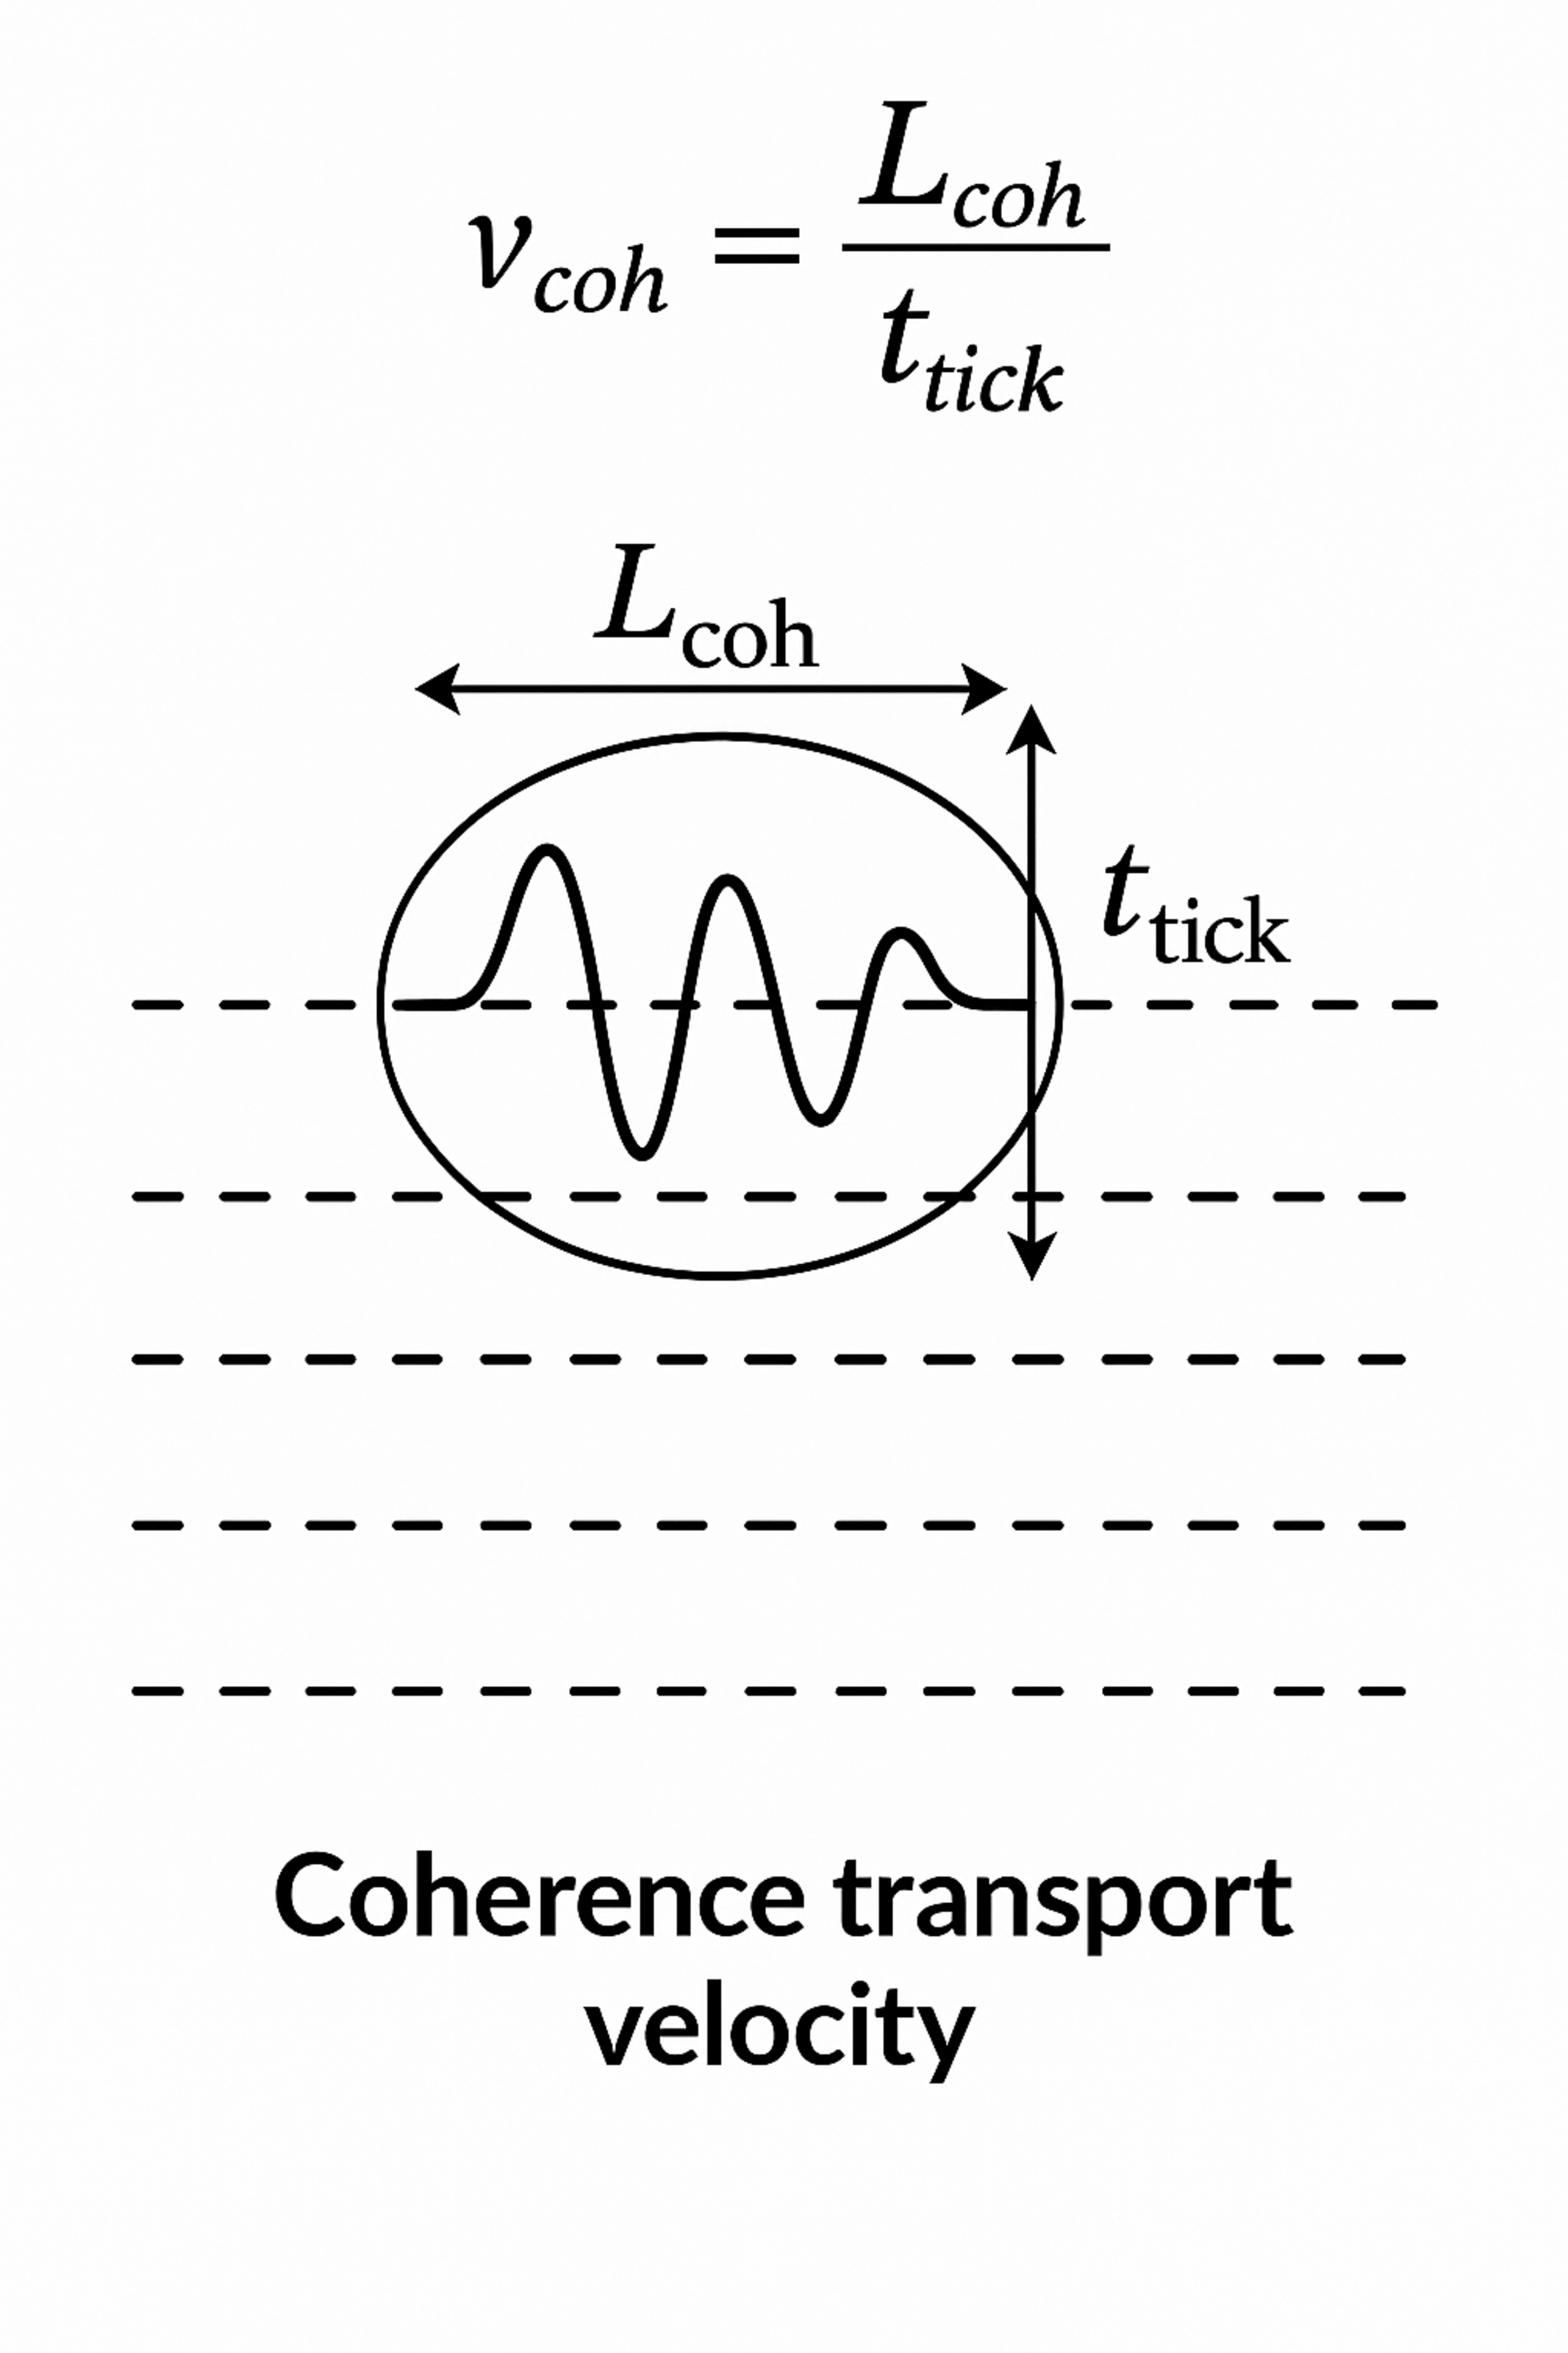
\includegraphics[width=0.6\textwidth]{figures/CTV.pdf}
    \caption{
    \textbf{Coherence Transport Velocity.} 
    In Quantum Substrate Dynamics (QSD), motion is governed not by geometric traversal, but by scalar-paced re-locking of coherence structures across the substrate. The coherence transport velocity is defined as \( v_{\text{coh}} = \frac{L_{\text{coh}}}{t_{\text{tick}}} \), where \( L_{\text{coh}} \) is the effective coherence envelope size and \( t_{\text{tick}} \) is the local scalar recovery interval. This expression sets the maximum apparent speed at which coherent structures can evolve through the substrate without violating causal re-locking constraints.
    }
    \label{fig:coherence-transport-velocity}
\end{figure}

This ontological shift enables a more physically grounded understanding of what it means for a structure to move, accelerate, or remain still. Stillness and uniform motion are no longer opposites—they are structurally indistinguishable in the absence of a substrate gradient. Motion only arises when reconfiguration is required under tension, and is experienced macroscopically as acceleration, inertia, and kinetic energy.


%%%%%%%%%%%%%%%%%%%%%%%%%%%%%%%%%%%%%%%%%%%%%%%%%%%%%%%%
\subsection{Inertia as Coherence Reconfiguration Resistance}

In classical physics, inertia is treated as an intrinsic property of mass—a passive resistance to acceleration. In the Quantum Substrate Dynamics (QSD) framework, inertia instead emerges from the substrate’s active resistance to the reconfiguration of a coherence structure. It is not the mass that resists motion, but the substrate that resists rapid or misaligned phase re-locking under causal pacing constraints.

A mass-phase structure is defined by a stable configuration of phase-locked scalar coherence within a conserved substrate region. When an external force attempts to accelerate this structure, it imposes a directional re-lock demand on the coherence boundary—pushing it to reconfigure into a new substrate region ahead of its causal pacing. This demand requires phase continuity across scalar gradients and is limited by the local re-locking rate—determined by the Planck-scale tick \( t_{\text{tick}} \). Inertia, then, is the scalar drag imposed by the substrate's recovery constraint: the energetic cost and delay associated with maintaining phase alignment during accelerated reconfiguration.

Mathematically, the inertial response can be modeled as a time-dependent resistance proportional to the local curvature and magnitude of the coherence phase gradient at the structure's boundary. Rather than viewing inertia as a fixed quantity tied to mass, QSD reframes it as a dynamic interaction: the more complex or tightly curved the boundary, the greater the resistance to re-locking, and thus the greater the observed inertia.

This interpretation naturally resolves the observed symmetry between acceleration and deceleration. In both cases, the substrate is being asked to alter the coherence path under time constraint—the direction is irrelevant to the underlying mechanism. The inertial experience is not due to momentum being lost or gained, but to scalar response lag when the substrate must deform structure under pacing limits.

By treating inertia as a reconfiguration process governed by scalar timing, QSD eliminates the need to treat mass as a fundamental entity. Instead, mass becomes a derived measure of how difficult it is to re-lock a given phase structure across the substrate. This interpretation preserves all classical and relativistic measurements while providing a substrate-level mechanism for resistance to motion.

To formalize this, we define a first-order inertial model based on local phase reconfiguration:

\begin{equation}
    F_{\text{inertial}} \propto \kappa \cdot \frac{d}{dt} \nabla \theta(\vec{r}),
\end{equation}

where \( \nabla \theta(\vec{r}) \) is the local phase gradient at the coherence boundary, and \( \kappa \) is a substrate compliance constant characterizing the resistance imposed by scalar recovery lag. This expression captures the dynamic structural response of the substrate to imposed acceleration under causal pacing.



%%%%%%%%%%%%%%%%%%%%%%%%%%%%%%%%%%%%%%%%%%
\subsection{Acceleration, Deceleration, and Momentum}

In the QSD framework, acceleration and deceleration are not fundamentally distinct phenomena. Both represent deviations from uniform scalar re-locking and require coherence reconfiguration. From the substrate's perspective, any change in motion imposes a new demand on the local phase gradient, leading to temporary deformation of the coherence shell. The direction of the change is irrelevant to the mechanism—what matters is that the substrate must reconfigure structure into a different alignment or pacing interval.

Momentum, in this view, is not a carried quantity but an expression of the substrate’s ongoing commitment to a reconfiguration path. It reflects the extent to which a coherence structure is already entangled with a directional scalar gradient. Once a system is in motion, the substrate has configured itself to support that coherence flow; interrupting or reversing it requires undoing that structural commitment.

Mathematically, momentum may be reinterpreted as the integral of scalar alignment over a coherence envelope:
\[
\vec{p}_{\text{QSD}} = \int_{\Omega} \rho(\vec{r}) \, \nabla \theta(\vec{r}) \, d^3r,
\]
where \( \rho(\vec{r}) \) is the local coherence density, and \( \nabla \theta(\vec{r}) \) is the phase gradient. This formulation captures both the directionality and accumulated substrate alignment of the mass-phase structure.

The energetic consequences of momentum are not stored in the object, but in the substrate’s geometric configuration. A sudden stop or impact results in scalar rupture: the substrate can no longer maintain coherence continuity and must offload tension as heat, vibration, or deformation. This resolves the classical paradox of energy release in collisions where no energy was apparently “stored.”

By reinterpreting acceleration, deceleration, and momentum as aspects of scalar reconfiguration within a conserved substrate, QSD offers a physically grounded mechanism for motion change. It preserves Newtonian behavior in its limit, while replacing axiomatic assumptions with structural causality.


%%%%%%%%%%%%%%%%%%%%%%%%%%%%%%%%%%%%%%%%%%
\subsection{Reinterpretation of Weight as Substrate Equilibrium Resistance}

In classical mechanics, weight is defined as the gravitational force acting on a mass: \( W = mg \), where \( g \) is the local field strength. This expression describes what is measured, but does not explain what weight is in structural terms. In the QSD framework, weight emerges from the substrate’s scalar tension gradient and the coherence structure’s resistance to being re-anchored into a lower-tension equilibrium.

Gravity in QSD is not a force field, but a coherence tension gradient within the substrate. Mass-phase structures immersed in such a gradient experience a directional preference for scalar re-locking toward regions of lower tension. Free-falling objects follow this gradient naturally, undergoing continuous re-locking without resistance. No internal deformation occurs—and thus no weight is perceived (see Figure~\ref{fig:weight-denied-relock}).

\begin{figure}[H]
    \centering
    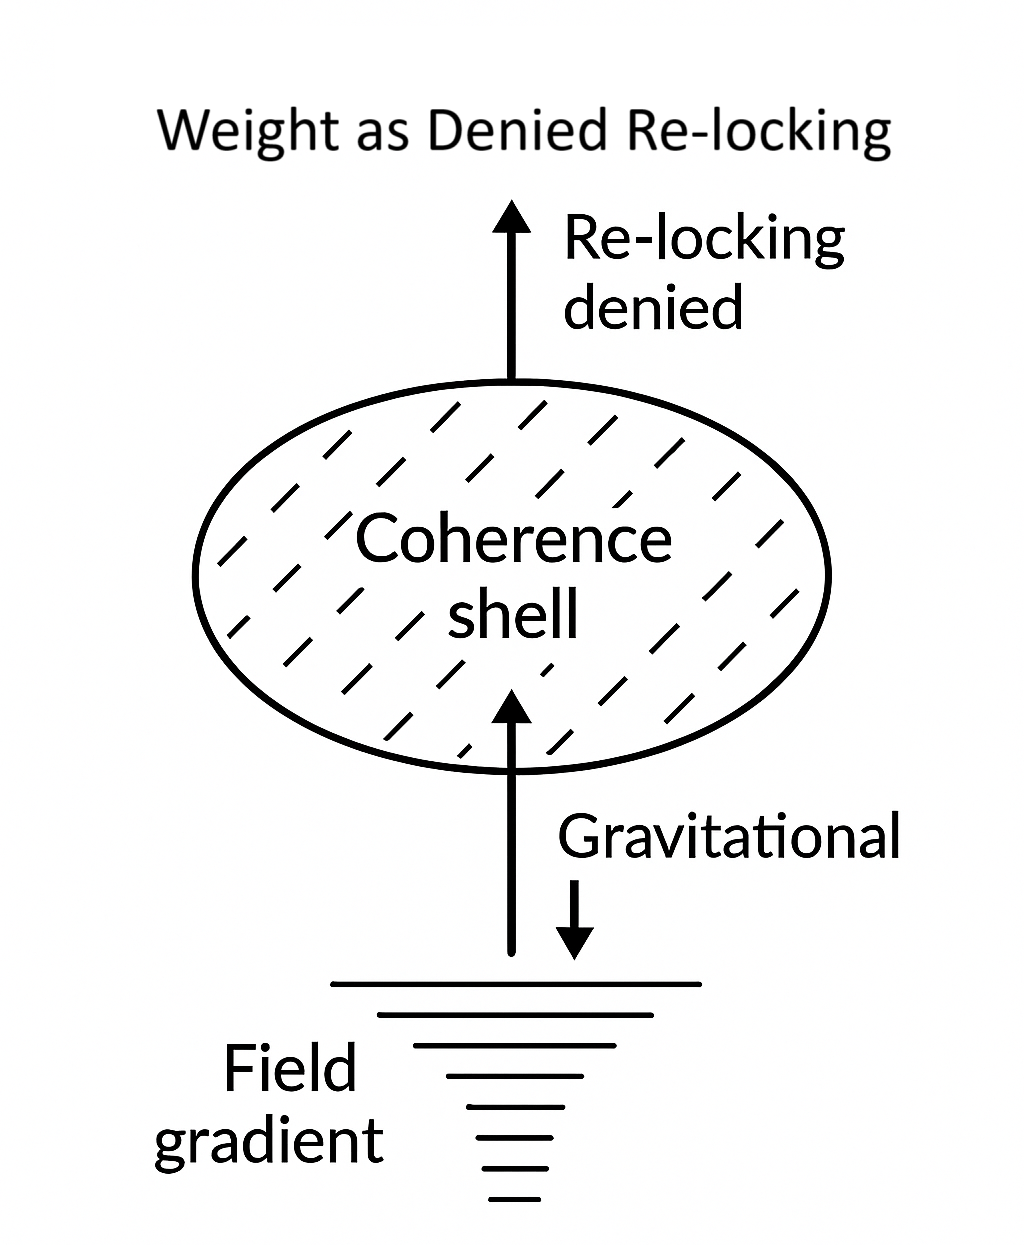
\includegraphics[width=0.5\textwidth]{figures/weight.png}
    \caption{
    \textbf{Weight as Denied Re-locking.}
    In the QSD framework, weight is not a force between masses but a structural phenomenon arising from coherence denial. A mass-phase coherence shell situated in a gravitational gradient attempts to re-lock into regions of lower scalar tension. When external constraints prevent this re-locking—such as contact with a surface—the substrate imposes a pushback against the denied direction. This denied reconfiguration manifests as weight: a scalar resistance to unfulfilled re-locking across a gradient. The gravitational vector reflects the substrate’s structural preference for re-lock alignment toward equilibrium.
    }
    \label{fig:weight-denied-relock}
\end{figure}

Weight only appears when re-locking is obstructed—such as when a structure is supported against the gradient by a surface. In this case, the substrate continues to attempt re-locking the coherence envelope downward, but tension cannot be resolved due to physical constraint. The result is a persistent scalar pushback, experienced macroscopically as weight. It is not a force transmitted through space, but a substrate tension response to denied coherence alignment.

This model naturally explains why free-falling bodies feel weightless: their coherence is re-locking continuously with the gradient without resistance. It also explains why astronauts in orbit experience microgravity despite remaining in Earth’s field—their mass-phase structures are in uninterrupted scalar descent and experience no obstruction.

In QSD, weight is not an intrinsic interaction between masses, but a local phenomenon arising from the interruption of coherence resolution. It scales with both the steepness of the scalar tension gradient and the structure’s reconfiguration difficulty. This interpretation grounds the sensation of weight in substrate dynamics and causal conservation.

This mechanism also reframes gravitational interaction without invoking attractive forces. A mass-phase structure deforms the substrate, introducing a coherence tension gradient. This gradient represents stored strain energy the substrate seeks to resolve. When another structure enters this gradient, it tends to re-lock toward lower-tension regions—not due to attraction, but because the substrate permits reconfiguration in the direction of lowest deformation cost. Motion in a gravitational field, then, is driven not by external force, but by internal coherence realignment.

To formalize this substrate-based origin of weight, we define the scalar pushback integral:

\begin{equation}
    W = \int_{\Omega} \rho(\vec{r}) \cdot \nabla \Phi_{\text{coh}}(\vec{r}) \, d^3r,
\end{equation}

where \( \rho(\vec{r}) \) is the coherence density, and \( \Phi_{\text{coh}}(\vec{r}) \) is the scalar coherence potential describing substrate tension alignment. This expression captures the substrate’s attempt to resolve a coherence structure into equilibrium and formalizes weight as the local response to denied scalar re-locking.

In this view, Newton’s second law is not discarded, but reinterpreted as a large-scale approximation of substrate resistance to coherence reconfiguration. The classical formulation \( F = ma \) becomes a surface-level expression of the structural tension that arises when a mass-phase structure is denied realignment with a scalar gradient. Acceleration does not result from force acting on mass, but from a directional increase in re-locking demand. When reconfiguration is obstructed—such as when an object is held against gravity—the substrate imposes a pushback proportional to both the gradient steepness (\( \nabla \Phi_{\text{coh}} \)) and the structure’s resistance to scalar adjustment. Force, then, is the substrate’s effort to complete a denied re-lock, and mass is the structural difficulty of doing so.

This perspective preserves classical outcomes while revealing their structural origin: weight is not a gravitational force, but a persistent tension from blocked substrate reconfiguration.



%%%%%%%%%%%%%%%%%%%%%%%%%%%%%%%%%%%%%%%%%%
\subsection{Rotation and Angular Momentum}

Within classical mechanics, angular momentum is treated as a conserved quantity: the product of a body’s moment of inertia and its angular velocity. This approach successfully predicts macroscopic rotational behavior, but offers no structural account of what angular momentum is or why rotating systems resist directional change. In Quantum Substrate Dynamics (QSD), angular momentum arises from the substrate’s conservation of curved phase flow. A rotating mass-phase structure induces persistent coherence deformation, and angular momentum is the measure of the substrate’s ongoing commitment to maintain this curved re-locking path.

Rotation differs fundamentally from linear motion. In uniform linear motion, scalar re-locking can occur without tension imbalance if the substrate gradient is flat. In contrast, rotation imposes continuous curvature on the coherence shell, requiring re-locking into geometrically misaligned adjacent zones. This re-locking under curvature creates structural strain in the substrate, which resists rapid change and demands scalar recovery to maintain.

The substrate stores this deformation as a standing torsional pattern—a curved memory—and any attempt to alter the rotation axis results in additional reconfiguration demand. This explains gyroscopic resistance: the substrate is actively conserving the angular phase geometry, and directional change requires it to restructure the coherence loop, which is energetically expensive.

Angular momentum in QSD is not a vector carried by the object, but a structural flow of phase within the substrate:
\[
\vec{L}_{\text{QSD}} = \int_{\Omega} \rho(\vec{r}) \left( \vec{r} \times \nabla \theta(\vec{r}) \right) d^3r,
\]
where \( \rho(\vec{r}) \) is the coherence density and \( \nabla \theta(\vec{r}) \) is the local phase gradient tangent to the curved motion path. This integral reflects the stored angular deformation, not just a kinematic property of mass.

Rotational behavior in QSD scales across all levels of physical structure. Whether in gyroscopes or spin-polarized subatomic structures, the substrate must preserve angular coherence continuity. The same substrate memory that resists tilting a spinning flywheel also governs the behavior of aligned spins in atomic or quantum systems. This suggests that macroscopic and microscopic rotational phenomena share a single origin: the conserved curvature of scalar re-locking within a coherence-bound medium.

Rotational motion also introduces persistent scalar recovery lag. The substrate cannot instantly recover from curved re-locking cycles, and this results in energy offload over time. Even uniform rotation leads to measurable thermal loss due to scalar rupture and jitter at the coherence boundary. Rapid directional changes, such as tilting a spinning gyroscope, accelerate this offload process, causing faster spin-down and increased heating—effects not explained by classical friction models.

The scalar recovery lag resulting from persistent curved motion can be modeled as an offload power function:

\begin{equation}
    P_{\text{offload}}(t) = \gamma \cdot \frac{\Delta E_{\text{torsion}}}{\tau},
\end{equation}

where \( \Delta E_{\text{torsion}} \) is the accumulated torsional strain energy stored in the coherence structure, \( \tau \) is the scalar recovery timescale, and \( \gamma \) is a coupling factor relating tension offload to measurable thermal output. This relationship provides a falsifiable prediction: that post-rotation heating scales with coherence strain and scalar pacing lag, even in isolated systems.

In QSD, angular momentum is structurally conserved but energetically costly. The longer or faster a body spins, the more curvature memory is invested in the substrate, and the more difficult it becomes to alter or interrupt that motion. This reframe explains gyroscopic stability, spin decay, and inertial resistance from first principles—without invoking mass as a primitive or relying on abstract conservation axioms (see Figure~\ref{fig:inertial-resistance}).

\begin{figure}[H]
    \centering
    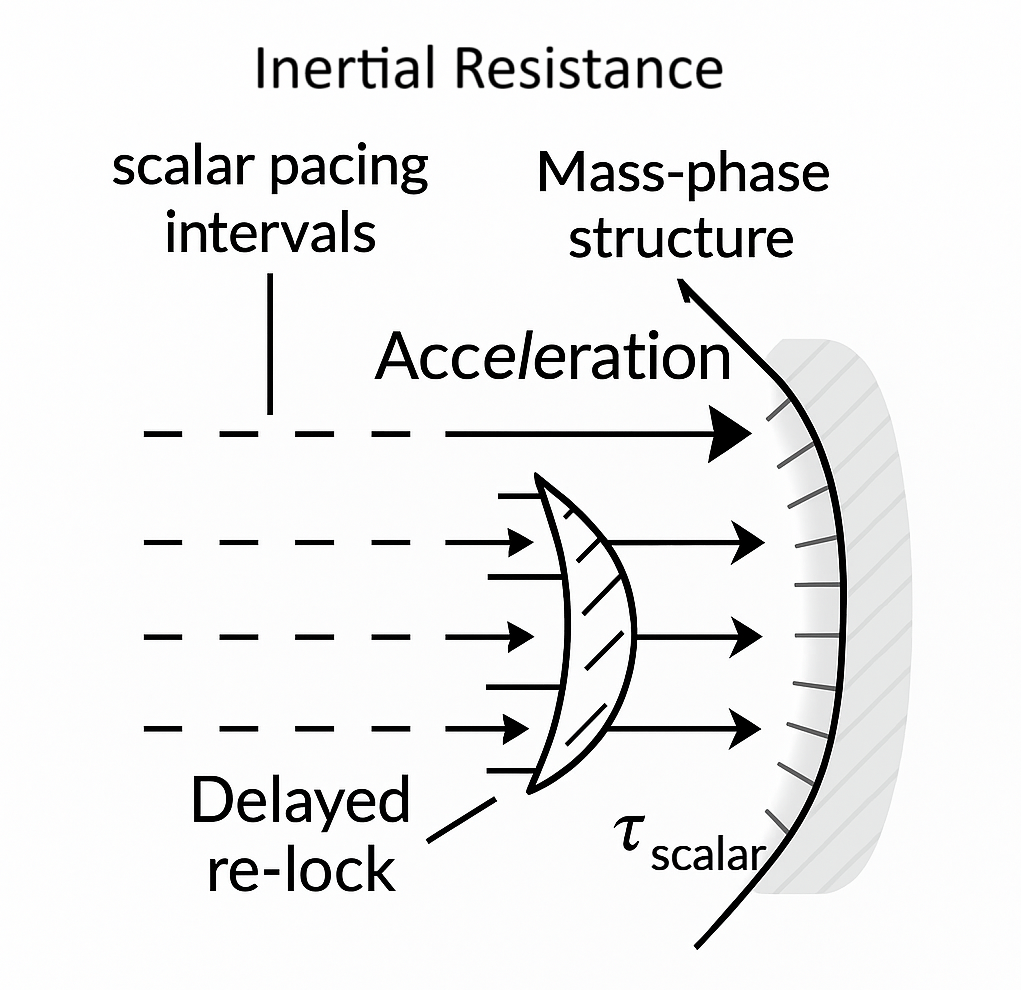
\includegraphics[width=0.6\textwidth]{figures/inertia.png}
    \caption{
    \textbf{Inertial Resistance and Scalar Pacing.}
    In Quantum Substrate Dynamics (QSD), inertial resistance arises from the delay between scalar pacing intervals and the structural reconfiguration of a mass-phase boundary. As a coherence structure accelerates, its re-locking into the substrate becomes desynchronized, resulting in a temporary lag or deformation. This delay, represented by the scalar recovery time \( \tau_{\text{scalar}} \), defines the pacing-limited resistance experienced as inertia. The substrate cannot re-lock the boundary faster than its causal capacity permits, making inertia a time-constrained response rather than an intrinsic mass property.
    }
    \label{fig:inertial-resistance}
\end{figure}

%%%%%%%%%%%%%%%%%%%%%%%%%%%%%%%%%%%%%%%%%%
\subsection{Energy and Motion}

In classical physics, energy is treated as a transferable, conserved quantity that can be stored in objects as kinetic or potential forms. Within the QSD framework, energy is reinterpreted not as a stored substance, but as the procedural act of reconfiguring phase-coherent structures within the substrate. All energetic behavior arises when coherence boundaries are deformed, displaced, or re-locked under scalar tension constraints.

Motion itself does not inherently carry energy. A coherence structure moving uniformly along a tension-neutral scalar gradient induces no substrate deformation and requires no offload. In such cases, the motion is structurally continuous and energetically silent. Energy expenditure arises only when motion changes—through acceleration, deceleration, rotation, or any event that disrupts uniform re-locking. These changes require the substrate to apply structural effort to preserve phase continuity, or to recover from misaligned re-locking.

In this view, kinetic energy is not something “possessed” by a moving object. It reflects the amount of tension the substrate must sustain to maintain coherence during non-neutral motion. Potential energy is similarly reframed: it is not stored in spatial position, but expresses the substrate’s readiness to resolve a mass-phase structure into a lower-tension configuration—such as when held above a gravitational gradient.

Thermal energy emerges when re-locking fails to occur cleanly. Scalar offload events dissipate residual tension as low-scale coherence jitter, which manifests macroscopically as heat. This explains why mechanical systems warm under repeated deformation—even in frictionless environments. The substrate's scalar memory saturates, forcing offload to maintain structural coherence.

Energy conservation in QSD is preserved structurally. What appears as conserved energy is the continuous redistribution of scalar tension and recovery effort. When a mass-phase structure comes to rest, its “lost” energy is not stored or annihilated—it has been offloaded into the substrate via structural reconfiguration and scalar delay. This provides a physical mechanism for transformation and dissipation without invoking abstract fields or hidden energy reservoirs.

QSD thus reframes energy as an emergent behavior of substrate tension management. Motion is energetically neutral unless it requires structural change. Only when coherence must be actively preserved against curvature, acceleration, or opposition does the substrate incur a cost. Energy is not something stored in moving things—it is what the substrate pays to keep coherence intact.


%%%%%%%%%%%%%%%%%%%%%%%%%%%%%%%%%%%%%%%%%%
\subsection{Compatibility with Classical Physics}

The Quantum Substrate Dynamics (QSD) framework reinterprets motion, inertia, and energy as structural outcomes of scalar coherence dynamics rather than as primitive concepts. Despite this ontological shift, QSD remains fully compatible with classical physics in its predictive domain. Classical equations of motion, Newtonian mechanics, and relativistic kinematics all emerge as effective summaries of substrate behavior in the appropriate limits.

QSD preserves conservation laws—including energy, momentum, and angular momentum—but reframes them as expressions of coherence preservation and substrate symmetry. Inertial reference frame equivalence, as formulated by Einstein, arises naturally from the substrate’s scalar neutrality in tension-balanced regions. Lorentz invariance is upheld through the scalar recovery constraint, which enforces causal propagation and ensures that no coherence structure can exceed the substrate’s re-locking rate.

Apparent paradoxes in classical motion—such as the equivalence of rest and uniform velocity, the energetic consequences of impact, and the origin of inertial resistance—are resolved structurally in QSD without altering observed behavior. Newton’s laws are recovered as large-scale expressions of substrate response: force emerges from imposed curvature, acceleration from reconfiguration demand, and mass from phase resistance geometry.

General relativity’s treatment of gravity as spacetime curvature finds a coherent analog in QSD: gravitational effects arise from scalar tension gradients within a conserved coherence field. This results in equivalent predictions for orbital motion, free fall, and gravitational time dilation, while offering a mechanism rooted in phase continuity rather than geometric postulation.

Importantly, QSD does not negate classical or quantum frameworks, but provides a deeper substrate from which their behaviors can be causally derived. It respects the successes of legacy physics while supplying structural explanations for quantities previously treated as axiomatic or abstract. In this way, QSD maintains continuity with established theory while extending its conceptual foundation to include causally coherent, falsifiable mechanisms.

%%%%%%%%%%%%%%%%%%%%%%%%%%%%%%%%%%%%%%%%%%
\subsection{Reframing Motion Through Structure}

The results presented in this work invite a fundamental shift in how motion, inertia, and momentum are understood—not as axiomatic quantities, but as emergent behaviors arising from phase-coherent structures embedded in a conserved substrate. The QSD framework offers a physically grounded mechanism for phenomena that classical and relativistic models treat as primitive: inertia becomes coherence drag, motion becomes scalar-paced re-locking, and momentum becomes the substrate’s directional commitment to maintaining structural continuity.

This reframing does not reject existing physics, but reveals the continuity beneath it. Classical laws remain valid as large-scale summaries, and relativistic constraints are preserved through the causal limits imposed by scalar recovery. The strength of the QSD approach lies in its ability to assign structural meaning to otherwise unexplained postulates—offering causal explanations for inertial resistance, the indistinguishability of rest and uniform motion, and the symmetry between acceleration and deceleration.

The framework also provides new interpretations for thermal effects and apparent energy loss in rotating systems. Scalar offload during coherence reconfiguration leads to measurable heating, even in vacuum environments—an effect often attributed to internal damping without a structural cause. QSD reveals that this heat arises from incomplete scalar recovery under persistent curvature, and predicts that rotating systems will exhibit asymmetric thermal signatures after directional changes, proportional to angular strain and tilt frequency.

More broadly, by placing coherence structure at the foundation of all motion, QSD suggests that even mass and energy are not intrinsic properties, but procedural outcomes of how the substrate stores and resolves phase tension. This has implications not only for classical dynamics, but for how quantum behavior, field interactions, and spacetime geometry are modeled at their most fundamental level.

This work represents a step toward a more physically transparent formulation of motion—one rooted not in abstract force but in substrate logic. It opens the door to new experimental programs, including scalar-based inertial sensing, post-rotation thermal mapping, and coherence-aligned transport mechanisms. The aim is not to discard the tools of modern physics, but to ground them in a unified substrate framework in which motion, inertia, and structure are inseparable aspects of a single conserved reality.

%%%%%%%%%%%%%%%%%%%%%%%%%%%%%%%%%%%%%%%%%%%
\section{Conclusion}
%%%%%%%%%%%%%%%%%%%%%%%%%%%%%%%%%%%%%%%%%%%
This work has presented a structural derivation of motion, inertia, and momentum under the framework of General Substrate Theory (GST), using the dynamic principles of Quantum Substrate Dynamics (QSD). By modeling mass-phase structures as phase-stable coherence knots embedded in a conserved substrate, we have shown that motion is not geometric traversal, but a sequence of scalar-paced re-locking events governed by a minimum causal interval—the Planck-scale tick. Inertia emerges from the substrate’s resistance to accelerated reconfiguration, momentum reflects the coherence already committed to a re-locking path, and weight arises from denied alignment with a scalar gradient.

Rotational motion was shown to impose persistent curvature strain on the substrate, producing irreversible scalar offload and thermal dissipation—even in the absence of classical friction. Angular momentum is reinterpreted as conserved phase curvature, and gyroscopic resistance emerges as the substrate’s structural commitment to preserving coherence geometry under rotation. These effects are not appended to physics—they are revealed as deeper substrate responses beneath familiar macroscopic and quantum behaviors.

Classical laws are preserved, but reinterpreted as emergent approximations of coherence structure evolving under causal constraint. Motion, stillness, and resistance are no longer distinct categories—they are continuous expressions of scalar re-locking dynamics. This work reframes Newtonian and relativistic behaviors as surface-level expressions of a deeper substrate ontology in which coherence, timing, and structural commitment define all observable dynamics.

This reinterpretation enables new approaches to modeling mechanical systems, inertial asymmetry, and thermally coupled motion from first principles. It provides a physical explanation for post-rotation heating, scalar recovery lag, and memory-linked inertial resistance. It also lays the groundwork for future investigations into coherence-bound transport, substrate-sensing technologies, and scalar-informed quantum behavior. By rooting motion in Planck-paced reconfiguration, General Substrate Theory offers a causally coherent and physically testable foundation—one in which motion, inertia, and structure are inseparable consequences of conserved coherence in an active substrate.





%%%%%%%%%%%%%%%%%%%%%%%%%%%%%%%%%%%%%%%%%%
\vspace{6pt} 

%%%%%%%%%%%%%%%%%%%%%%%%%%%%%%%%%%%%%%%%%%
%% optional
%\supplementary{The following supporting information can be downloaded at:  \linksupplementary{s1}, Figure S1: title; Table S1: title; Video S1: title.}

% Only for journal Methods and Protocols:
% If you wish to submit a video article, please do so with any other supplementary material.
% \supplementary{The following supporting information can be downloaded at: \linksupplementary{s1}, Figure S1: title; Table S1: title; Video S1: title. A supporting video article is available at doi: link.}

% Only used for preprtints:
% \supplementary{The following supporting information can be downloaded at the website of this paper posted on \href{https://www.preprints.org/}{Preprints.org}.}

% Only for journal Hardware:
% If you wish to submit a video article, please do so with any other supplementary material.
% \supplementary{The following supporting information can be downloaded at: \linksupplementary{s1}, Figure S1: title; Table S1: title; Video S1: title.\vspace{6pt}\\
%\begin{tabularx}{\textwidth}{lll}
%\toprule
%\textbf{Name} & \textbf{Type} & \textbf{Description} \\
%\midrule
%S1 & Python script (.py) & Script of python source code used in XX \\
%S2 & Text (.txt) & Script of modelling code used to make Figure X \\
%S3 & Text (.txt) & Raw data from experiment X \\
%S4 & Video (.mp4) & Video demonstrating the hardware in use \\
%... & ... & ... \\
%\bottomrule
%\end{tabularx}
%}

\section*{Statements and Declarations}
\subsection*{Funding}  
The author received no financial support for the research, authorship, or publication of this article.
The author has no relevant financial or non-financial interests to disclose.

\subsection*{Competing Interests}  
The author declares no competing interests.

\subsection*{Author Contributions}  
The author solely conceived, developed, and wrote the manuscript, including all theoretical content, references, and formatting.

\subsection*{Data Availability}  
No datasets were generated or analyzed during the current study. All references are publicly available.

\subsection*{Ethical Approval}  
Not applicable.


%%%%%%%%%%%%%%%%%%%%%%%%%%%%%%%%%%%%%%%%%%
%% Optional

%% Only for journal Encyclopedia
%\entrylink{The Link to this entry published on the encyclopedia platform.}

\abbreviations{Abbreviations}{
The following abbreviations are used in this manuscript:
\\

\noindent
\begin{tabular}{@{}ll}
QSD   & Quantum Substrate Dynamics \\
\( c_s \) & Scalar coherence recovery speed (temporal mode) \\
\( c_t \) & Transverse coherence propagation speed (spatial mode) \\
\( L_0 \) & Baseline coherence length at rest \\
\( L_{\text{coh}}(r) \) & Curvature-stretched coherence support length \\
\( v \) & Apparent velocity relative to substrate \\
\( v_{\text{coh}} \) & Coherence transport velocity \( = \frac{L_{\text{coh}}}{t_{\text{tick}}} \) \\
\( t_{\text{tick}} \) & Local scalar recovery interval (effective time tick) \\
\( t_0 \) & Tick duration at rest (baseline tick) \\
\( \kappa \) & Substrate compliance constant (resistance to boundary deformation) \\
\( \theta(\vec{r}) \) & Local coherence phase at position \( \vec{r} \) \\
\( \rho(\vec{r}) \) & Coherence density distribution \\
\( F_{\text{inertial}} \) & Inertial response force under reconfiguration stress \\
\( P_{\text{offload}}(t) \) & Scalar thermal offload power over time \\
\( \Delta E_{\text{torsion}} \) & Accumulated torsional energy due to rotational strain \\
\( \tau \) & Scalar recovery lag timescale \\
\( \gamma \) & Lorentz factor (compatible structural form) \\
GPS  & Global Positioning System \\
SR   & Special Relativity \\
GR   & General Relativity \\
\end{tabular}

}



%%%%%%%%%%%%%%%%%%%%%%%%%%%%%%%%%%%%%%%%%%
%% Optional
\appendixtitles{no} % Leave argument "no" if all appendix headings stay EMPTY (then no dot is printed after "Appendix A"). If the appendix sections contain a heading then change the argument to "yes".
\appendixstart
\appendix
%%%%%%%%%%%%%%%%%%%%%%%%%%%%%%%%%%%%%%%%%%%%%%%
\section[\appendixname~\thesection]{}
\subsection[\appendixname~\thesubsection]{Canonical QSD Motion Equations}
%%%%%%%%%%%%%%%%%%%%%%%%%%%%%%%%%%%%%%%%%%%%%%
The following expressions summarize the core structural relationships introduced in this paper. Each equation reflects a substrate-level mechanism associated with motion, inertia, momentum, thermal offload, or gravitational resistance, redefined within the Quantum Substrate Dynamics (QSD) framework.

\subsubsection{Inertial Resistance}
Inertia arises from the substrate’s opposition to accelerated boundary reconfiguration under phase-gradient strain:
\begin{equation}
    F_{\text{inertial}} \propto \kappa \cdot \frac{d}{dt} \nabla \theta(\vec{r}),
\end{equation}
where \( \kappa \) is the substrate compliance constant and \( \nabla \theta(\vec{r}) \) is the local phase gradient at the coherence boundary.

\subsubsection{Momentum as Coherence Path Commitment}
Momentum reflects the directional coherence alignment stored across a mass-phase structure:
\begin{equation}
    \vec{p}_{\text{QSD}} = \int_{\Omega} \rho(\vec{r}) \, \nabla \theta(\vec{r}) \, d^3r,
\end{equation}
where \( \rho(\vec{r}) \) is the local coherence density and \( \nabla \theta(\vec{r}) \) is the phase gradient describing structural alignment.

\subsubsection{Rotational Offload Power}
Rotational strain induces scalar recovery lag, leading to thermal offload as curvature accumulates:
\begin{equation}
    P_{\text{offload}}(t) = \gamma \cdot \frac{\Delta E_{\text{torsion}}}{\tau},
\end{equation}
where \( \Delta E_{\text{torsion}} \) is the accumulated torsional strain energy, \( \tau \) is the scalar recovery timescale, and \( \gamma \) is a coupling constant relating strain to offload rate.

\subsubsection{Weight from Gradient Tension}
Weight arises from substrate pushback when scalar re-locking is obstructed within a gravitational coherence gradient:
\begin{equation}
    W = \int_{\Omega} \rho(\vec{r}) \cdot \nabla \Phi_{\text{coh}}(\vec{r}) \, d^3r,
\end{equation}
where \( \Phi_{\text{coh}}(\vec{r}) \) is the coherence tension potential and \( \rho(\vec{r}) \) is the structure’s coherence density.

\subsubsection{Coherence Transport Velocity}
The velocity of motion is constrained by the pacing limit of scalar re-locking, not geometric traversal:
\begin{equation}
    v_{\text{coh}} = \frac{L_{\text{coh}}}{t_{\text{tick}}},
\end{equation}
where \( L_{\text{coh}} \) is the coherence envelope size and \( t_{\text{tick}} \) is the local scalar recovery interval.

\vspace{1em}

These expressions serve as the foundational mechanics for motion in the QSD framework. Each replaces classical kinematic assumptions with a structurally grounded description of motion as a coherence process governed by causal timing, geometric strain, and substrate conservation.


%%%%%%%%%%%%%%%%%%%%%%%%%%%%%%%%%%%%%%%%%%%%%%

%%%%%%%%%%%%%%%%%%%%%%%%%%%%%%%%%%%%%%
%\subsubsection{SUB A}
%%%%%%%%%%%%%%%%%%%%%%%%%%%%%%%%%%%%%%

%%%%%%%%%%%%%%%%%%%%%%%%%%%%%%%%%%%%%%%%%%%%%%%
%\section[\appendixname~\thesection]{}
%\subsection[\appendixname~\thesubsection]{APP B}
%%%%%%%%%%%%%%%%%%%%%%%%%%%%%%%%%%%%%%%%%%%%%%%

%\subsubsection{SUB B}

%%%%%%%%%%%%%%%%%%%%%%%%%%%%%%%%%%%%%%%%%%
%\isPreprints{} % If the paper is ``preprints'', please uncomment this parenthesis.
%\printendnotes[custom] % Un-comment to print a list of endnotes

\reftitle{References}

% Please provide either the correct journal abbreviation (e.g. according to the “List of Title Word Abbreviations” http://www.issn.org/services/online-services/access-to-the-ltwa/) or the full name of the journal.
% Citations and References in Supplementary files are permitted provided that they also appear in the reference list here. 

%=====================================
% References, variant A: external bibliography
%=====================================
% \bibliography{your_external_BibTeX_file}

%=====================================
% References, variant B: internal bibliography
%=====================================

% ACS format
\isAPAandChicago{}{%
\begin{thebibliography}{999}
% Reference 
\bibitem{bush2025}
\textbf{Preprint.} Bush, M. (2025). Quantum Substrate Dynamics (QSD): A Relativistic Field Model of Emergent Mass, Inertia and Gravity. \textit{Preprints}, 2025060988. \url{https://doi.org/10.20944/preprints202506.0988.v1}
% reference
\bibitem{bush-planck-2025}
\textbf{Preprint.} Bush, M. (2025). Planck’s Constant Physically Derived Through Quantum Substrate Dynamics: A Mode-Ratio and Offload-Based Origin for Quantization and Temporal Structure. \textit{Preprints}, 2024010211. \url{https://doi.org/10.20944/preprints202401.0211.v1}
% Reference 
\bibitem{bush-coherence}
Bush, M. The Coherence Envelope: Defining the Minimum Structural Unit of Action in Quantum Substrate Dynamics. {\em Preprints} {\bf 2025}, \url{https://doi.org/10.20944/preprints202506.2353.v1}.
% Reference 
\bibitem{bush-planck-ep}
Bush, M. Planck Energy as Collapse Limit: A Structural Interpretation of $E_P$ in Quantum Substrate Dynamics. {\em Preprints} {\bf 2025}, \url{https://doi.org/10.20944/preprints202507.0080.v1}.
% Reference 
\bibitem[Ashby(2003)]{ashby-gps}
Ashby, N. Relativity in the Global Positioning System. {\em Living Rev. Relativ.} {\bf 2003}, {\em 6}, 1--50. \url{https://doi.org/10.12942/lrr-2003-1}.
% Reference
\bibitem[Bailey et al.(1977)]{bailey-muon}
Bailey, J.; Borer, K.; Combley, F.; Drumm, H.; Krienen, F.; Picasso, E.; von Ruden, W.; Farley, F.J.M.; Field, J.H. Measurements of relativistic time dilatation for positive and negative muons in a circular orbit. {\em Nature} {\bf 1977}, {\em 268}, 301--305. \url{https://doi.org/10.1038/268301a0}.
% reference
\bibitem[Everitt et al.(2011)]{gp-b}
Everitt, C.W.F.; et al. Gravity Probe B: Final Results of a Space Experiment to Test General Relativity. {\em Phys. Rev. Lett.} {\bf 2011}, {\em 106}, 221101. \url{https://doi.org/10.1103/PhysRevLett.106.221101}.

\bibitem[Chua et al.(2018)]{rotational-heating}
Chua, S.K.; et al. Thermal Noise in Precision Rotational Measurements. {\em Rev. Sci. Instrum.} {\bf 2018}, {\em 89}, 104501. \url{https://doi.org/10.1063/1.5042276}.


\end{thebibliography}
}

% Chicago format (Used for journal: arts, genealogy, histories, humanities, jintelligence, laws, literature, religions, risks, socsci)
\isChicagoStyle{%
\begin{thebibliography}{999}
% Reference 1
%\bibitem[Aranceta-Bartrina(1999a)]{ref-journal}
%Aranceta-Bartrina, Javier. 1999a. Title of the cited article. \textit{Journal Title} %6: 100--10.
% Reference 2

\end{thebibliography}
}{}

% APA format (Used for journal: admsci, behavsci, businesses, econometrics, economies, education, ejihpe, games, humans, ijfs, journalmedia, jrfm, languages, psycholint, publications, tourismhosp, youth)
\isAPAStyle{%
\begin{thebibliography}{999}
% Reference 1
%\bibitem[\protect\citeauthoryear{Azikiwe \BBA\ Bello}{{2020a}}]{ref-journal}
%Azikiwe, H., \& Bello, A. (2020a). Title of the cited article. \textit{Journal Title}, \textit{Volume}(Issue), 
%Firstpage--Lastpage/Article Number.

\end{thebibliography}
}{}

% If authors have biography, please use the format below
%\section*{Short Biography of Authors}
%\bio
%{\raisebox{-0.35cm}{\includegraphics[width=3.5cm,height=5.3cm,clip,keepaspectratio]{Definitions/author1.pdf}}}
%{\textbf{Firstname Lastname} Biography of first author}
%
%\bio
%{\raisebox{-0.35cm}{\includegraphics[width=3.5cm,height=5.3cm,clip,keepaspectratio]{Definitions/author2.jpg}}}
%{\textbf{Firstname Lastname} Biography of second author}

% For the MDPI journals use author-date citation, please follow the formatting guidelines on http://www.mdpi.com/authors/references
% To cite two works by the same author: \citeauthor{ref-journal-1a} (\citeyear{ref-journal-1a}, \citeyear{ref-journal-1b}). This produces: Whittaker (1967, 1975)
% To cite two works by the same author with specific pages: \citeauthor{ref-journal-3a} (\citeyear{ref-journal-3a}, p. 328; \citeyear{ref-journal-3b}, p.475). This produces: Wong (1999, p. 328; 2000, p. 475)

%%%%%%%%%%%%%%%%%%%%%%%%%%%%%%%%%%%%%%%%%%
%% for journal Sci
%\reviewreports{\\
%Reviewer 1 comments and authors’ response\\
%Reviewer 2 comments and authors’ response\\
%Reviewer 3 comments and authors’ response
%}
%%%%%%%%%%%%%%%%%%%%%%%%%%%%%%%%%%%%%%%%%%
\PublishersNote{}
%\isPreprints{} % If the paper is ``preprints'', please uncomment this parenthesis.
\end{document}

